\chapter{Background \& Related Work}
\label{ch:background}

In this section we introduce the background necessary to understand the context of the project, and explore some related works which we utilise and build upon.

\section{Interfaces in Embedded Systems}
\label{sec:embedded-interfaces}

Interfacing between digital components is hard due to high speed and precision timing requirements, and is a problem continually explored by electronics engineers.

\subsection{Consumer Hardware}
In consumer electronics the USB interface is common, and devices include hardware USB controllers to handle the timing and signalling required to understand each other properly. On a desktop or laptop computer other interfaces such as SATA and PCIe can be found, which handle communication with internal peripherals such as hard drives and expansion cards like GPUs.

Performance and timing accuracy is key in such applications, as consumers want their systems to be responsive and reliable. Dedicated interface hardware that is specialised for each protocol is standard in consumer systems, as it allows the CPU to continue to perform other tasks while I/O happens in the background. Communicaton between the CPU and I/O hardware usually happens via interrupts, shared memory, and/or DMA, all coordinated by system software usually within an OS kernel.

\subsection{Embedded Systems}

Microcontrollers and embedded systems are similar in that they included dedicated I/O hardware, but interfaces like SATA are rarely found on an MCU. Instead, interfaces such as SPI, UART, I\textsuperscript{2}C, PWM, CAN are more common, along with GPIO pins. These interfaces are more general-purpose, and designed for use with other electronic components rather than consumer hardware. They're also are a lot simpler than the likes of PCIe, and easy to implement into a small microcontroller fairly cheaply \cite{rp2040}.

This is suitable for most use cases, but the issue still remains that designers have a fixed and limited range of hardware to choose from. It is often the case that a device does not include a specific interface that is needed, or has too many of one interface and not enough of another. Some more exotic peripherals may also include custom interfaces (to quote Raspbery Pi, `cursed serial devices found on AliExpress`) which are not supported in any of the existing hardware.

As an example, Espressif's ESP32 is one of the most popular microcontrollers on the market at the moment, due to a combination of its low cost and WiFi \& Bluetooth capabilities. In terms of digital I/O hardware, the device has 3 UART interfaces, two I\textsuperscript{2}C buses, two I\textsuperscript{2}S buses, three SPIs, a PWM controller, a TWAI/CAN (Two Wire Automotive Interface) controller, an SDIO/SPI slave controller, and an SD/SDIO/MMC host controller \cite{esp32}. This is a broad complement of I/O hardware that is representative of most devices on the market, but if a designer did want to connect more than three SPI devices, or a peripheral that doesn't support one of the aforementioned protocols, then they are left in a difficult situation.

One solution to this is to use the processing system of a microcontroller to read/write to the GPIO pins at high speeds to implement the required signalling such that the external hardware can understand the data. This is a technique known as `bit-banging', and is very hard because CPUs are not designed for this, and usually cannot meet the precise timing requirements of external devices. Programmers often write very tight loops of assembly code in the hope that the CPU will execute their instructions on the exact cycle that they want them to, but with the increasing complexity of modern CPUs and the advent of out-of-order architectures, this is increasingly rare. CPU time is also precious in embedded systems, and bit-banging consumes lots of power and processor cycles \cite{bitbang}.

\subsection{FPGAs}

The proper solution to custom interface requirements is custom hardware, but this can be very expensive. Designing a custom microprocessor and getting it manufactured can cost hundreds of thousands if not millions, and is not practical to do in small quantities. The field-programmable gate array, or FPGA is another solution: semiconductors containing a matrix of configurable logic cells based around a programmable interconnect network that can be configured to implement arbitrary logic circuits. FPGAs are very flexible, and capable of high I/O throughput with absolute precision and control. However, they can be very expensive, an order of magnitude more than most low-cost microcontrollers. FPGAs also present a very unique programming model which may be unfamiliar to most software engineers, making them hard to work with \cite{whatisfpga}.

Embedded systems including FPGAs are not uncommon for high-performance or highly custom applications: Xilinx's Zynq-7000 SoCs combine programmable logic with two ARM Cortex-A9 CPU cores as shown in Figure \ref{fig:zynq}. The SoC also includes standard external interfaces such as I\textsuperscript{2}C and SPI, but can be programmed to add additional interfaces through the programmable logic subsystem \cite{zynq}.

\begin{figure}[H]
    \centering
    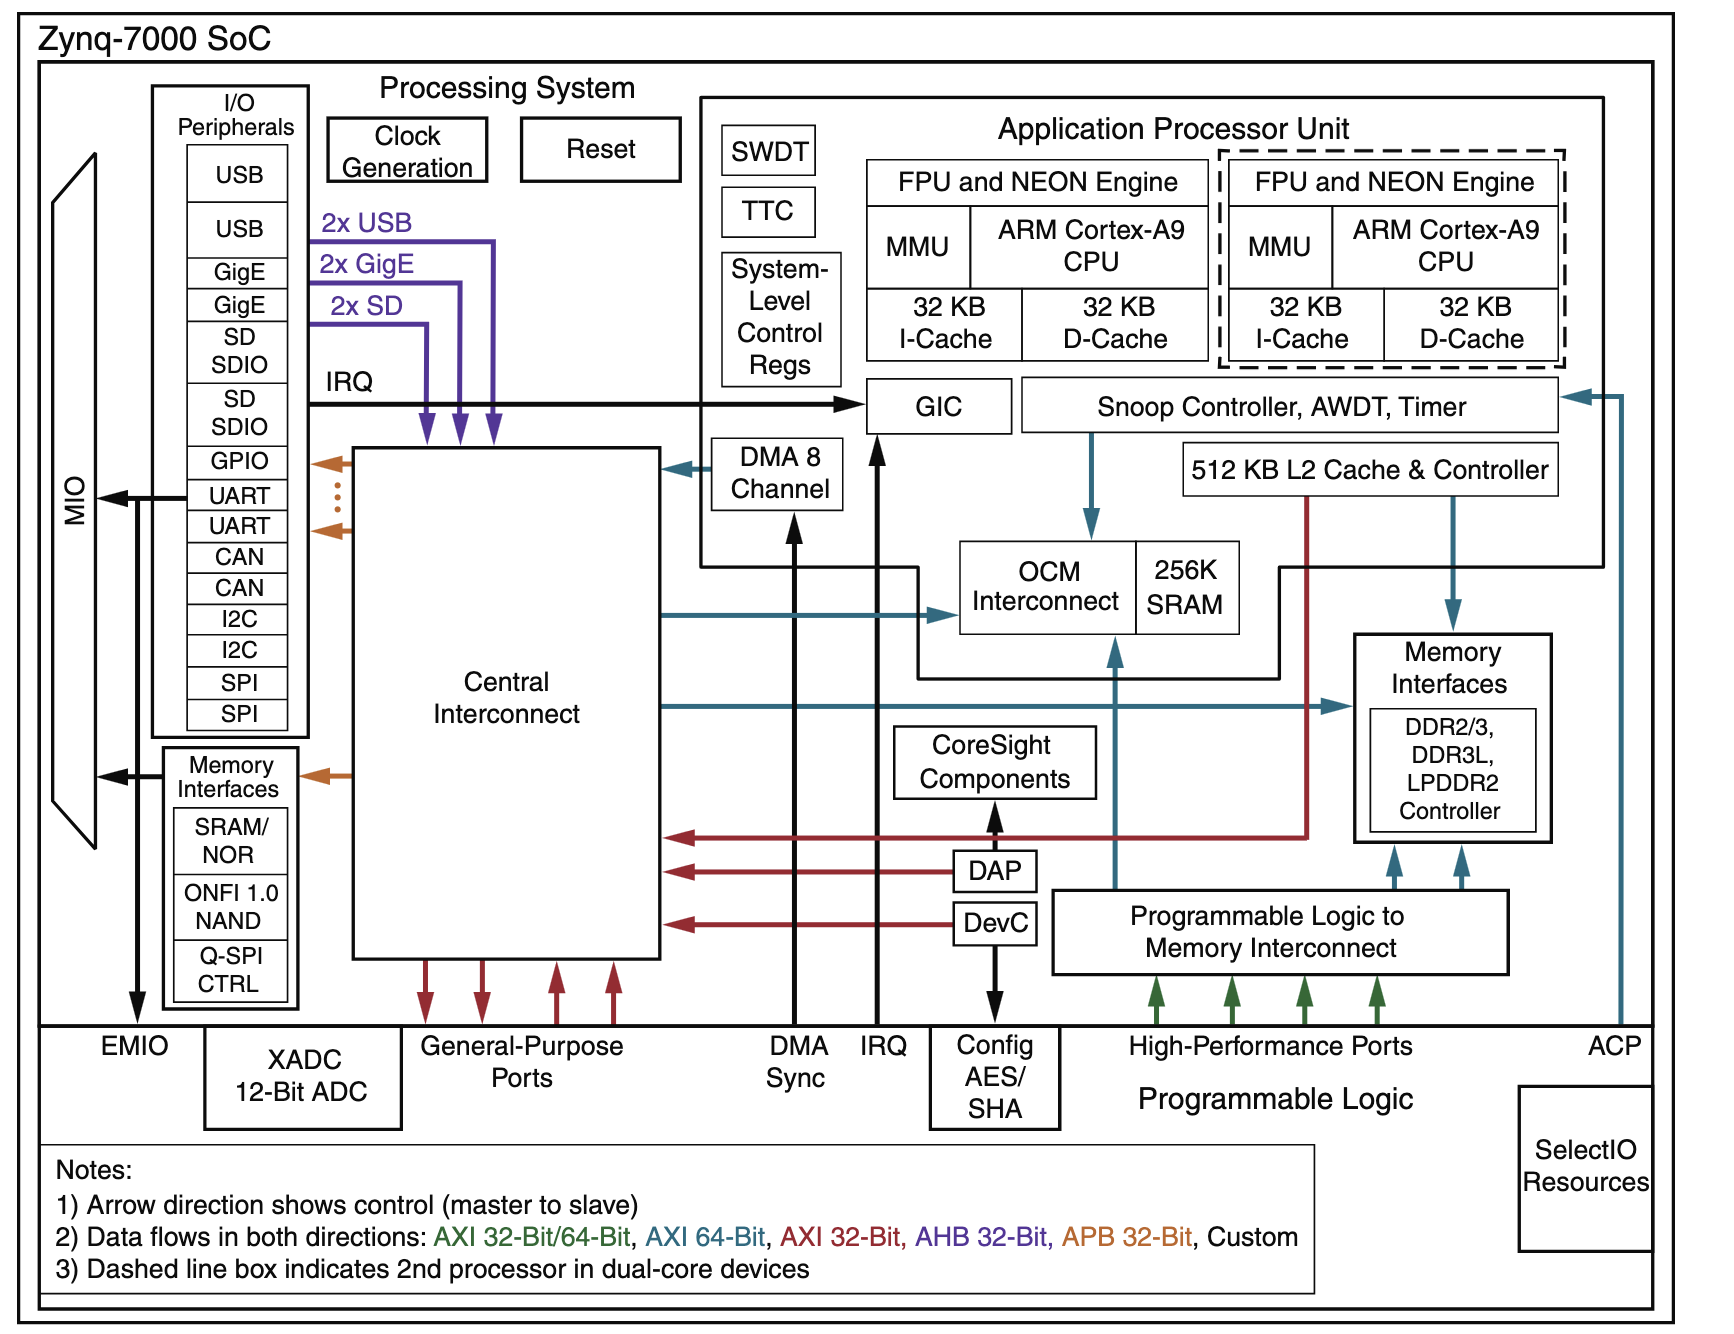
\includegraphics[width=0.85\textwidth]{../img/zynq.png}
    \caption{Block diagram of Xilinx's Zynq-7000 Architecture \cite{zynq}}
    \label{fig:zynq}
\end{figure}

A novel reconfigurable I/O interface using FPGAs is presented by Aibe and Yasunaga in \cite{metaio}. They attempt to solve a similar problem to PIO, but utilise an FPGA with multiple bitstreams stored in a ROM, such that the interface can then reconfigure the FPGA to act as a controller for whatever device is currently connected. This is a similar approach the the Zynq SoC, combining fixed hardware with programmable logic, but different in that they propose a full interface standard based around the technique for mobile and consumer electronics.

\section{The RP2040 and PIO}
Raspberry Pi acknowledge the issues mentioned in Chapter \ref{ch:introduction} and Section \ref{sec:embedded-interfaces} in their introduction to the RP2040's PIO in their documentation, pitching it as a way to add additional hardware interfaces to a device without the drawbacks of bit-banging or programmable logic. PIO is fixed-function hardware included in the RP2040 with a similar power draw and chip area utilisation to a typical embedded hardware interface such as a UART or SPI controller, built to operate with cycle-accuracy and determinism at up to 48MHz (the system clock speed), allowing it to meet the timing requirements necessary for many high-speed serial interfaces \cite{rp2040}.

Figure \ref{fig:pio-sm} gives an overview of one of the PIO state machines. Included in each one are two 32-bit shift registers, two 32-bit scratch registers, a clock divider, flexible GPIO pin mapping, and 2 4x32-bit FIFOs connected to the system bus. Each PIO block includes 4 state machines, each capable of executing independently. The architecture is designed to perform a small set of operations, primarily setting/clearing GPIO pins, and moving data to/from the processor (optionally using the DMA subsystem) \cite{rp2040}.

\begin{figure}[H]
    \centering
    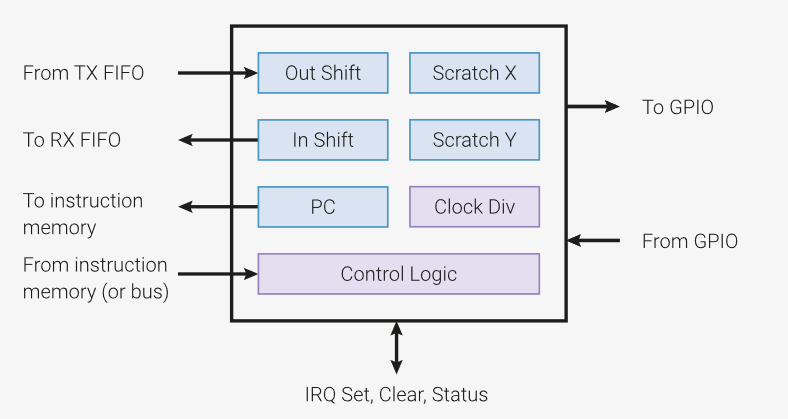
\includegraphics[width=0.7\textwidth]{../img/rp2040-state-machine.png}
    \caption{An overview of a PIO State Machine \citep{rp2040}}
    \label{fig:pio-sm}
\end{figure}

The flexibility and power of the PIO blocks allow them to be programmed to implement common interfaces such as UART and SPI, more complex interfaces such as DVI and SDIO, and even custom interfaces to enable tight integration with other external hardware in bespoke embedded systems.

The RP2040 PIO is programmable via a small assembly-like language called PIO assembly, or pioasm. It contains only 9 instructions, each executed within a single clock cycle. The instruction set is very dense: the PIO is capable of sampling a GPIO pin, toggling an output clock, and pushing a data word to the system all with a single instruction. An small example program is shown in Listing \ref{lst:sqwave} that outputs a square wave on a single GPIO pin. The example uses only 2 of the 9 instructions: \mintinline{text}|set| to drive GPIO pins, and \mintinline{text}|jmp| to implement a loop. More details on pioasm is given in Chapter \ref{ch:design} as part of our design discussion.

\begin{listing}[H]
    \vspace{0.5cm}
    \begin{minted}{asm}
set pindirs, 1   ; Set pin to output
again:
set pins, 1 [1]  ; Drive pin high, delay for one cycle
set pins, 0      ; Drive pin low
jmp again        ; Set PC to label `again`
    \end{minted}
    \caption{PIO Assembly to output a square wave \citep{rp2040}}
    \label{lst:sqwave}
\end{listing}


\section{I/O Coprocessors}
The idea of offloading I/O to a coprocessor is not novel. We explore two other devices which include subsystems that are designed for I/O.
\subsection{Time Processor Unit}

The Time Processor Unit (TPU) is a coprocessing subsystem found in some older Motorola microcontrollers \cite{tpu}, built upon by the Enhanced TPU (eTPU) in NXP Semiconductor's MCF523x family of microcontrollers built on the ColdFire architecture \cite{mfcdatasheet}.

The eTPU is a real-time microprocessed system, designed to run microengine code on a built-in RISC processor to respond to events triggered by either internal timers, interrupts, or I/O transitions. Each eTPU engine consists of 32 channels, each with an input and output and containing logic to listen for up to 4 events. Channels can be independently configured to perform functions such as output generation, input capture, or a combination of the two. The eTPU is designed for control of system timing operations and for I/O control. It is capable of implementing UART and SPI, as well as more specialised protocols for motor control and automotive applications.

Communication between the eTPU and host CPU happens via a shared RAM, which can be used for data transfer between the two and as storage for eTPU microcode programs. The CPU configures the eTPU by writing to the relevant configuration registers within the system's address space, and can configure each channel mode and priority independently \cite{etpu}.

The event-driven architecture differs from that of the RP2040's PIO, in that timing is decoupled from the microcode execution: code is executed in response to an event, rather than the timing being built in to the execution of the code. However, the guarantees provided by the hardware around event response latency and the nature of microcode execution within the TPU means it can meet the timing requirements necessary for interfaces such as UART. The eTPU's included RISC processor means it presents a more familiar programming model than the RP2040's state machines to software engineers, and provides a much broader set of operations.

\subsection{ESP-32 Ultra Low Power Coprocessor}

The ESP-32 contains an ultra-low power coprocessor (ULP) that can remain powered on when the rest of the SoC is in deep sleep mode. The ULP is a finite state machine can execute a program from it's own memory that is capable of accessing peripheral devices and internal sensors, and communicating via I\textsuperscript{2}C. It can wake the CPU and send interrupts to the host system, as well as control it's own sleep state. It can communicate with the rest of the SoC via a shared memory that can be read/written by the ULP while the rest of the SoC is in deep sleep. It can be started directly by software on the host system, or by a hardware timer triggered periodically.

The ULP is also based around a state machine like the RP2040, and programmable using assembly. However, the ULP's assembly language is much more featured than the PIO, with a full ALU and support for load/store operations to a shared system memory similar to the eTPU. The ULP is also programmable via a set of macros in C, which makes it much more accessible than the RP2040 and eTPU. Unlike PIO and the eTPU, the ULP is not designed to implement arbitrary I/O protocols, instead acting as a co-processor that has access to only I\textsuperscript{2}C, ADC and GPIO interface hardware. Instead, it's purpose is to offload I/O functions from the CPU to save power. Given the ESP32 positioning itself as an IoT microcontroller, this makes sense, as IoT devices often want to consume as little power as possible \cite{esp32}.

Despite this, the idea of an I/O-focused coprocessor designed to operate in ultra-low power states is powerful. IoT devices often operate on tightly contstrained power budgets, and as battery-powered embedded systems become more prevalent in applications such as wearables and wireless devices, the need for I/O at low power is evident.


\begin{table}[h!]
    \centering
    \begin{tabular}{|p{0.2\linewidth}|p{0.2\linewidth}|p{0.25\linewidth}|p{0.25\linewidth}|}
        \hline
        \textbf{Device}            & \textbf{PIO}         & \textbf{eTPU}                 & \textbf{ULP}                         \\ \hline
        \textbf{Programming model} & Specialised assembly & RISC assembly                 & Specialised assembly or C/C++ macros \\ \hline
        \textbf{Architecture}      & State machine        & Event-driven, RISC processor  & State machine                        \\ \hline
        \textbf{Purpose}           & Arbitrary I/O        & Timing control, arbitrary I/O & Low power IoT functions              \\ \hline
        \textbf{Flexibility}       & High                 & Medium                        & Low                                  \\ \hline
    \end{tabular}
    \caption{A comparison of PIO, eTPU and ULP features.}
    \label{tab:comparison}
\end{table}

\section{RISC-V}

RISC-V is an open standard instruction set architecture. Originally developed at the University of California, Berkely to support computer architecture research and education, it has grown into an industry standard and is being used in commercial devices. RISC-V was designed explicitly to be an open standard ISA, but also to be `a \textit{real} ISA' \cite{riscv_design}, such that it would be suitable for hardware implementation in an FPGA or ASIC. It was also designed to be highly flexible and extensible, a factor showcased by it's many extension standards \cite{riscv_spec}.

RISC-V is supported in many important open-source software projects, including the Linux kernel, system toolchains such as LLVM and GNU GCC, libc and binutils, emulators such as QEMU and Spike, as well as other programming languages such as Rust and Go \cite{riscv_wiki}.

This support has allow for RISC-V to become a viable option for hardware vendors to manufacture commercial offerings. SiFive, a startup founded by three of RISC-V's creators, was one of the first companies to design and manufacture RISC-V silicon, but bigger companies including Google and Western Digital are now investing heavily in RISC-V \cite{riscv_article}.

We utilise RISC-V for this project: it's open source nature means it is free for us to use and experiment with. It was designed from the start to be microarchitecture-agnostic, which means there are many well-supported open source implementations are available. It's flexibility also means it is possible to easily and closely integrate external peripherals.

\subsection{Rocket Chip}

Rocket chip is one such implementation. Rocket chip is an open source library of hardware components that provides an generator framework for building custom RISC-V SoCs. The framework includes two RISC-V core types: the in-order Rocket Core, and out-of-order BOOM core. Rocket chip is parametrised extensively: the included cores themselves are configurable with different pipelines and functional units, and the larger system can be configured with different quantities and levels of cache and different interconnect mechanisms. Figure \ref{fig:rocket} shows an example design containing two `tiles' (Rocket's organisation of cache-coherent units), each with different CPU types, cache configurations and accelerators. An L2 cache is included, and an AXI4 bridge provides a mechanism for connecting external peripherals.

\begin{figure}[h!]
    \centering
    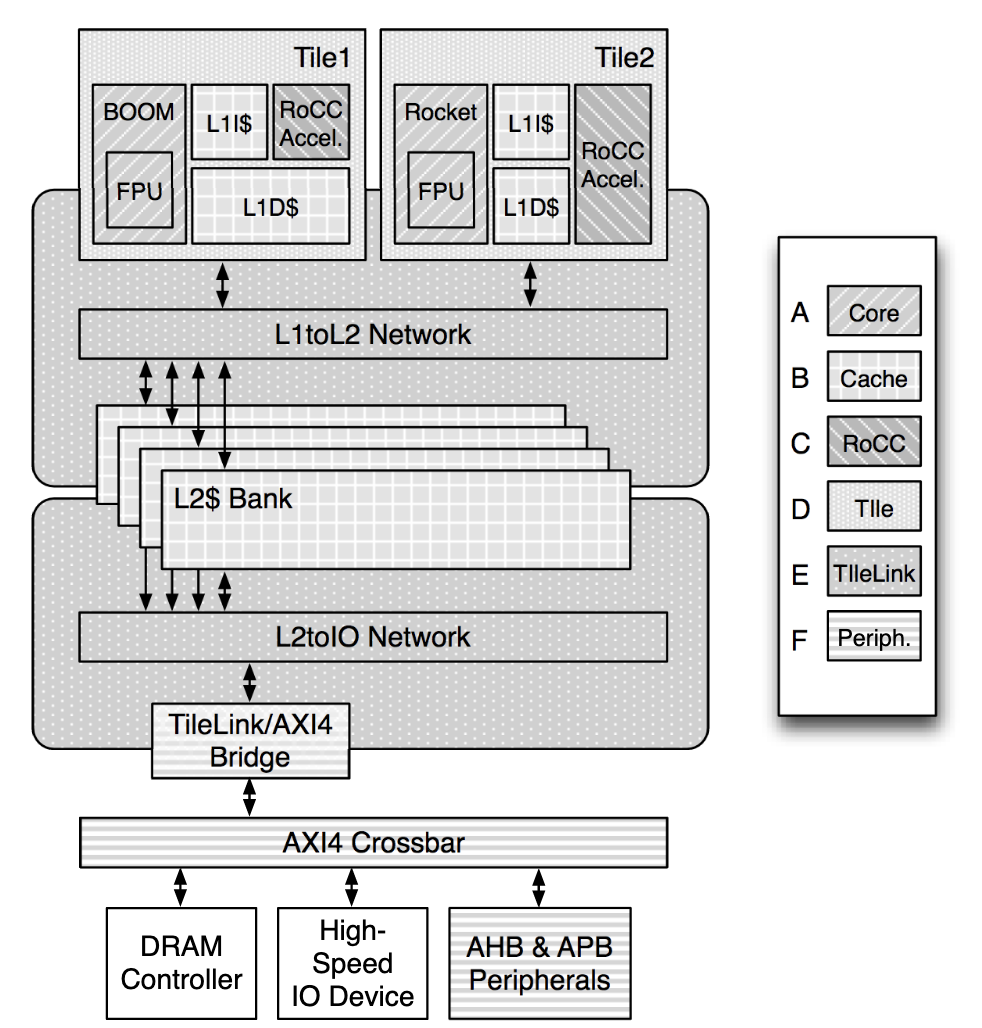
\includegraphics[width=0.7\textwidth]{../img/rocket-chip.png}
    \caption{An example Rocket chip design, showcasing it's sub-components~\cite{rocketchip}}
    \label{fig:rocket}
\end{figure}

Rocket chip provides multiple ways to integrate custom units: as custom RISC-V extensions directly within a core, as a coprocessor via the RoCC (Rocket Custom Coprocessor) interface, or fully decoupled and connected to the memory system via TileLink, the SoC interconnect. The ability to easily integrate custom units as closely as desired is ideal for this project and allows us to integrate PIO as closely as we desire.

The Rocket Core itself is a 5-stage\footnote{The pipeline is described as 5 stage in \cite{rocketchip}, but Figure \ref{fig:rocket-core} shows 6 stages. We believe that the PC stage is not counted.} in-order scalar core that implements the RV32G and RV64G specifications: the base 32 \& 64 bit RISC-V spec with the M (integer multiplication \& division), A (atomics), F (32-bit floating point), and D (64-bit floating point) extensions. It has an MMU that support page-based virtual memory, a non-blocking data cache, and a front-end with branch prediction. Configuration options exposed include the optional support of the extensions mentioned, the number of floating point pipeline stages, the cache and TLB sizes, and the branch prediction buffers and tables.

Rocket Chip is also a major component of Chipyard: an integrated SoC design, simulation and verification framework designed for agile development of specialised hardware. It includes Rocket Chip, but also accelerators such as the Hwacha vector unit generator and various domain-specific generators for cryptography, digital signal processing, and machine learning \cite{chipyard}.

\begin{figure}[h!]
    \centering
    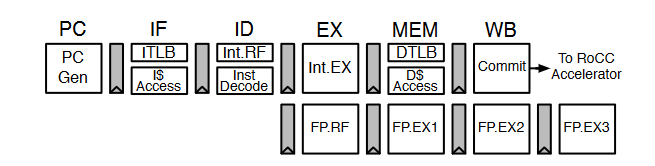
\includegraphics[width=0.9\textwidth]{../img/rocket-core.png}
    \caption{The Rocket core pipeline \cite{rocketchip} }
    \label{fig:rocket-core}
\end{figure}

\section{Chisel}
Rocket chip is written in Chisel, a hardware description language that supports hardware design with highly parametrised generators using a DSL embedded within Scala. It is through Chisel that Rocket Chip is able to provide such parametric hardware.

Verilog and VHDL, the two most popular HDLs, were originally designed as hardware \textit{simulation} languages in the 1980s and were only later adopted for \textit{synthesis}. Their semantics are such that design must be inferred from a subset of them, which complicates development of tooling and end usage. These languages are also very dated, lacking abstraction and typing features that are common in modern programming languages developed in the 21st century.

Chisel presents an alternative. As a set of Scala libraries providing facilities for hardware construction on the register transfer level, (RTL),  HDL modules can be written as Scala classes. It leverages Scala's strong type system to provide type-safe hardware construction using types such as \txt{Bool} and \txt{UInt} to represent single and multi-bit wires, as well as aggregate data types such as \txt{Bundle} and \txt{Vec} for collections of signals. Implicit parameters are used to abstract away clock and reset signals, simplifying hardware designs and allowing designers to focus on expressing logic. Polymorphic and parametric types allow for expressing hardware designs that are configurable both on the type and value level, raising the level of abstraction for hardware construction above what is possible in Verilog to create designs that allow for better code reuse and easier hardware design space exploration \cite{chisel}.

\begin{figure}[H]
    \centering
    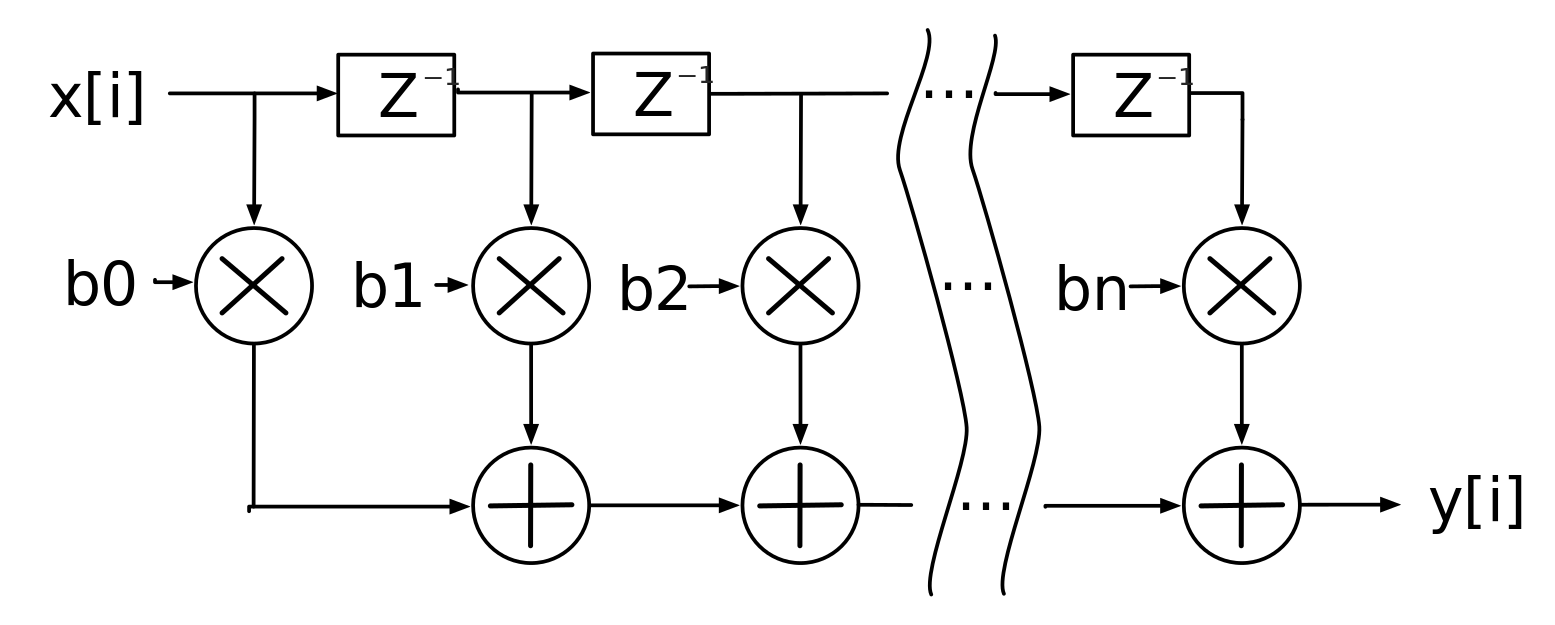
\includegraphics[width=0.9\textwidth]{../img/fir_filter.png}
    \caption{A multiply-accumulate FIR filter \cite{chisel_site}}
    \label{fig:fir}
\end{figure}

As an example, consider an arbitrary-length FIR filter implementing a convolution operation, as shown in Figure \ref{fig:fir}. Listing \ref{lst:chisel_fir} showcases how Chisel leverages Scala to provide parametric abstractions usable hardware. Scala's functional declarative style and standard library are match closely to the declarative style of hardware description, which makes for very succinct but expressive code.



\begin{listing}[H]
    \vspace{0.5cm}
    \begin{minted}{scala}
// parametrised by bit width (Int)
// and Scala list of hardware coefficients (Seq[UInt])
class FirFilter(bitWidth: Int, coeffs: Seq[UInt]) 
    extends Module {
    // one input and one output of this module
    val io = IO(new Bundle {
    val in = Input(UInt(bitWidth.W))
    val out = Output(UInt(bitWidth.W))
    })
    
    // the filter's length
    val N = coeffs.length

    // register that holds N UInts
    val zs = Reg(Vec(N, UInt(bitWidth.W)))
    // register driven by input
    zs(0) := io.in 
    // shift the register contents on each cycle 
    // clock implicit
    for (i <- 1 until coeffs.length) {
        zs(i) := zs(i-1)
    }

    // multiply the register with the coefficients
    val products = VecInit
        .tabulate(N)(i => zs(i) * coeffs(i))

    // Sum the products, drive the output
    io.out := products.reduce(_ + _)
}
    \end{minted}
    \caption{Code implementing the circuit shown in Figure \ref{fig:fir} \cite{chisel_site}}
    \label{lst:chisel_fir}
\end{listing}

Chisel has an ecosystem of tools surrounding it too, making it convenient to work with. It's libraries and compiler are built on FIRRTL (Flexible Intermediate Representation for Register Transfer Level), an intermediate representation designed for hardware description languages \cite{firrtl}. Native verification and simulation tools also exist: the ChiselTest library builds on existing Scala/JVM testing libraries to provide infrastructure for easily writing unit test-style testbenches for Chisel. ChiselTest uses Treadle, a high-performance native simulator and execution engine for FIRRTL that can be used for verification of hardware designs\footnote{\url{https://github.com/chipsalliance/treadle}}. Treadle also includes a REPL for ad-hoc interactive verification of designs, which can be very convenient for quick testing \cite{chisel_site}.

\section{Rust for Embedded Systems}

Bare-metal embedded software environments, such as the one we present in our SoC design, are constrained in resources and demand a higher level of control over the hardware than most application software. Typically, such software is written in C or C++, as other popular software languages such as Python or Java exist on too high a level of abstraction from the underlying hardware and require runtime software such as a garbage collector that adds additional overhead.

A viable alternative is Rust. Rust compiles directly to an executable binary with similar performance to C/C++, and provides zero-cost abstractions that allow for writing software on a higher level with no runtime overhead, making it suitable for embedded development. Rust's advantages lie in powerful static analysis that enforces memory safety at compile time, eliminating entire classes of errors that are common in C/C++ \cite{rust-paper}.

This is done via a mechanism known as the borrow checker. Built into the compiler, it enforces that only a single part of the program can mutate data at any point, and ensures that all data is valid when it is used. This prevents race conditions and memory bugs such as null pointer dereferencing and use-after-frees. Encapsulating and validating data access and enforcing read-only state helps to reason about programming with peripherals in a microcontroller, and provides a much more robust programming model than treating them as global mutable state \cite{rust-usability, rust-good}.

Rust's strong, functional type system allows for more expressive modelling of systems at compile time. As an example, GPIO pins can be configured into a number of states (enabled/disabled, input/output, pull-up/pull-down inputs), but only certain combinations of these states are valid. The state a pin is in also determines what operations are valid on it: you can't write data to an input pin. This can be modelled on the type level using typestate programming in Rust, as show in Listing \ref{lst:rust_gpio} \cite{embedded_rust}.

\begin{listing}[H]
    \vspace{0.5cm}
    \begin{minted}{rust}
/// GPIO interface
/// Type parameters encode configuration
struct GpioPin<ENABLED, DIRECTION>;

// Type states for configuration parameters
struct Disabled;
struct Enabled;
struct Output;
struct Input;

/// This function may be used on an enabled output Pin
/// &mut indicates mutation of state
impl GpioPin<Enabled, Output> {
    pub fn write_bit(&mut self) { ... }
}

/// This function may be used on an enabled input Pin
impl GpioPin<Enabled, Input> {
    pub fn read_bit(&self) -> bool { ... }
}

/// These functions may be used on a disabled pin
impl<DIR> GpioPin<Disabled, DIR> {
    pub fn into_enabled_output(self) 
        -> GpioPin::<Enabled, Output> { ... }
    pub fn into_enabled_input(self) 
        -> GpioPin::<Enabled, Input> { ... }
}
    \end{minted}
    \caption{Rust code modelling the state of a GPIO pin. Type parameters encode state at compile time, and \mintinline{text}|impl| blocks are parametrised to allow only valid transitions between states and prevent misuse of the API \cite{embedded_rust}.}
    \label{lst:rust_gpio}
\end{listing}

Support for RISC-V exists within the Rust compiler, and there is a \txt{riscv} library that provides low-level access to hardware devices and registers\footnote{\url{https://github.com/rust-embedded/riscv}}, along with other libraries designed for embedded development that are easy to use due to Rust's tight integration with it's build tool Cargo. We leverage the strong static guarantees and ecosystem support provided by Rust to implement software for testing our SoC design.

\section{FPGAs}

Usually, a microcontroller design such as the one we implement would be fabricated as an ASIC so it can be integrated into a board and other embedded systems. ASICs also provide much higher performance and efficiency than equivalent hardware implemented on FPGAs \cite{fpga_v_asic}. However, this is not an option for us as silicon fabrication is expensive and has to be done at scale. Instead, we target FPGAs for implementation, specifically a Xilinx Artix-7-100T device on a Digilent Nexys A7 board \cite{digilent}.

FPGAs contain logic and interconnect resources, designed to be reconfigured into arbitrary digital logic circuits. The primary fundamental unit of FPGA architecture is the configurable logic block (CLB). A Xilinx 7-series CLB contains 6-input lookup tables (LUTs), small memories that can be configured to implement arbitrary combinational logic, and flip-flops and latches that can implement sequential logic.

7-series devices also contain block RAMs and FIFOs that can be used to implement memory within a logic design. Memory can also be implemented as distributed RAM, or LUTRAM, which combines multiple LUTs together to implement memories \cite{fpga_arch}.

FPGAs are introduced in Section \ref{sec:embedded-interfaces} as I/O components in embedded systems, but they also provide an ideal platform for experimentation and verification. They are often used for prototyping hardware designs and for implementing proofs of concept such as ours.

\begin{figure}[h!]
    \centering
    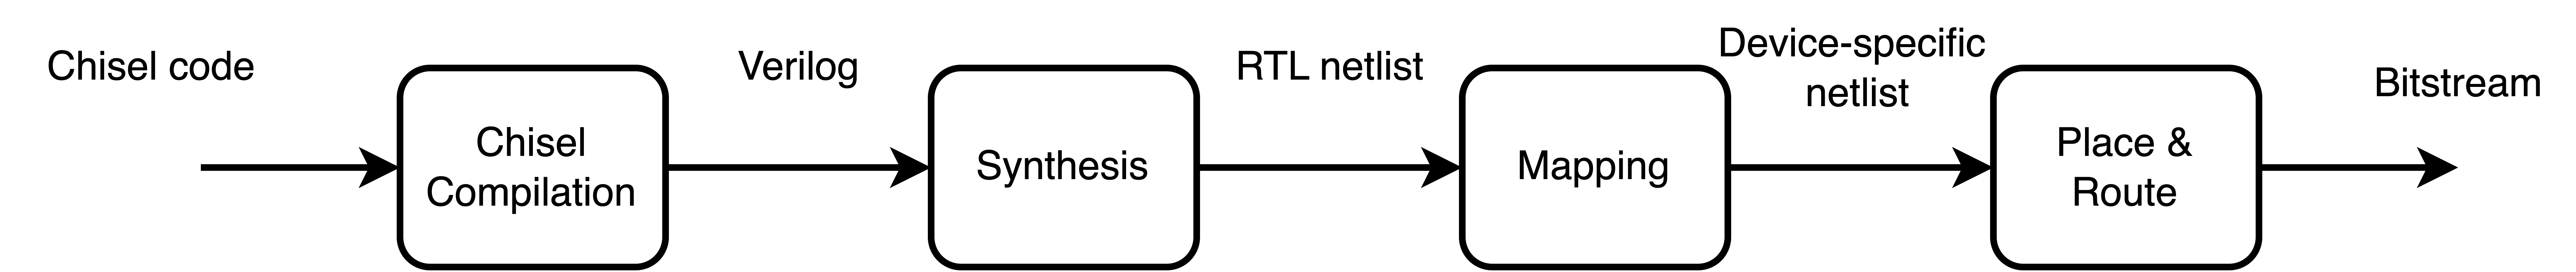
\includegraphics[width=\textwidth]{../img/design-flow.png}
    \caption{The FPGA design flow}
    \label{fig:design-flow}
\end{figure}

Hardware designs for FPGAs traditionally start as Verilog or VHDL code, which is then synthesised to a netlist of RTL components, then the place and route process maps the netlist to physical resources on the device and configures the interconnect. The configuration is saved to a file as a bitstream \cite{vivado_design}.

The way Chisel fits into the FPGA design flow is as an extra RTL compilation step prior to synthesis. The Chisel compiler compiles Chisel modules within Scala to Verilog modules which can then be synthesised the same as any other Verilog code. This allows for the reuse of existing FPGA tooling and workflows, as well as interoperability with Verilog codebases \cite{chisel}.

